该实验部分采用 REINFORCE 策略梯度算法~\cite{DBLP:journals/ml/Williams92} 对清扫机器人任务进行训练。

REINFORCE 算法是一种基于策略梯度的强化学习算法,用于求解策略优化问题。
它属于无模型强化学习算法,直接通过策略来选择动作并进行优化,而不是通过值函数或环境模型来估计动作的回报。
在传统的值函数方法(如 \(Q\)-Learning 或 SARSA)中,核心目标是学习一个状态-动作值函数 \(Q \left( s, a \right)\),再通过贪婪策略派生出最优行为。

但一般认为在复杂任务中,值函数方法往往不易收敛,且对连续动作空间支持不佳。为此,引入了 \textbf{策略梯度方法(Policy Gradient Methods)},直接建模并优化一个参数化策略 \(\pi_{\theta} \left( a \mid s \right) \),以提高学习的稳定性与泛化能力。
在这一基础上,Williams et al. 提出了 REINFORCE,这也是最早的、也是最简单的一种蒙特卡洛策略梯度算法。其核心思想是:
\begin{itemize}
    \item “利用完整轨迹中的实际奖励来指导策略的改进,增强出现好结果的动作概率,抑制差结果的动作。”
\end{itemize}

策略梯度的优化目标为最大化期望总回报:
\begin{equation}\label{eq:policy_gradient_objective}
    \mathbf{J} \left( \theta \right) = \mathbb{E}_{\tau \sim \pi_{\theta}} \left[ R \left( \tau \right) \right]
\end{equation}
其中,\(\tau = \left(s_0, a_0, r_1, \dots, s_T, a_T, r_{T+1}\right)\) 表示一个完整轨迹,\(R \left( \tau \right)\) 为轨迹总回报。
通过对数概率技巧(log-derivative trick),策略梯度可以表示为:
\begin{equation}\label{eq:policy_gradient-log}
    \nabla_{\theta} \mathbf{J} \left( \theta \right) = \mathbb{E}_{\tau \sim \pi_{\theta}} \left[ \sum_{\pi_\theta} \nabla_{\theta} \log \pi_{\theta} \left( a_t \mid s_t \right) \cdot R_t \right]
\end{equation}
其中 \(R_t\) 是从时刻 \(t\) 开始的累计折扣奖励:
\[
    R_t = \sum_{k=0}^{T-t} \gamma^k r_{t+k+1}
\]
这种形式意味着——在每一步中,提高当时策略选择该动作的概率,按当前回报加权。

REINFORCE 的梯度估计是无偏的,但由于直接用回报 \(R\) 乘以 \(\log\) 概率,导致方差较大,训练不稳定。
为此,常引入 baseline(基线) 来降低方差,所以公式 (\ref{eq:policy_gradient_objective}) 可以改写为:
\begin{equation}\label{eq:policy_gradient_objective-log_baseline}
    \mathbf{J} \left( \theta \right) = \nabla_{\theta} \mathbf{J} \left( \theta \right) = \mathbb{E}_{\tau \sim \pi_{\theta}} \left[ \sum_{\pi_\theta} \nabla_{\theta} \log \pi_{\theta} \left( a_t \mid s_t \right) \cdot \left( R_t - b_t \right) \right]
\end{equation}
在本文中,我们的实现就是如公式 (\ref{eq:policy_gradient_objective-log_baseline}) 加入了 baseline 的 REINFORCE 算法。
算法归纳参考算法~\ref{agl:REINFORCE_replay},其中包含熵正则项(Entropy Regularization)来鼓励策略的探索性,算法中参数的含义和具体实现参考后文中的小节~\ref{subsubsec:REINFORCE-state-action} 部分。

\begin{algorithm}[htbp]
\caption{REINFORCE 策略梯度算法}\label{agl:REINFORCE_replay}
\KwIn{
    策略网络 $\pi_\theta(a \mid s)$, 
    折扣因子 $\gamma$, 
    回放权重 $\beta$, 
    初始熵系数 $\lambda_{\texttt{init}}$, 
    最小熵系数 $\lambda_{\texttt{min}}$, 
    初始学习率 $\alpha_{\texttt{init}}$, 
    学习率衰减因子 $\kappa$($\kappa\in(0,1)$), 
    学习率衰减步数 $S$(每隔 $S$ 轮触发一次衰减), 
    最⼤训练轮数 $E$, 
    成功轨迹缓存上限 $N$, 
    重放频率 $K$, 
    固定最大步数上限 $T$
}
\KwOut{最优策略参数 \( \theta \)}

初始化成功轨迹缓存池:\( \mathcal{M} \leftarrow \emptyset \)\;
设置当前学习率 $\alpha \leftarrow \alpha_{\texttt{init}}$ \;

\For{\( \text{episode} = 1 \) \KwTo \( E \)}{
    初始化环境状态 \( s_0 \)\;
    初始化轨迹存储列表:\( S \leftarrow [] \),\( A \leftarrow [] \),\( R \leftarrow [] \)\;

    \While{未终止}{
        采样动作:\( a_t \sim \pi_\theta(\cdot \mid s_t) \)\;
        执行动作,获得奖励 \( r_t \) 和新状态 \( s_{t+1} \)\;
        记录:\( S \gets S \cup \{s_t\} \),\( A \gets A \cup \{a_t\} \),\( R \gets R \cup \{r_t\} \)\;
    }

    \If{ 成功拾取垃圾 }{
        将 \( (S, A, R) \) 存入成功缓存 \( \mathcal{M} \)\;
        若 \( |\mathcal{M}| > N \),则移除最旧轨迹\;
    }

    \For{\( t = 0 \) \KwTo \( T \)}{
        计算折扣回报:
        \[
        R_t \leftarrow \sum_{k=0}^{T - t} \gamma^k r_{t + k} ;
        \]
    }

    计算 baseline:
    \[
    \bar{R} = \frac{1}{T+1} \sum_{t=0}^T R_t \;
    \]
    \For{$t = 0$ \KwTo $T$}{
        计算 Advantage:
        \[  
        A_t \leftarrow \frac{\hat{A}_t - \mu}{\sigma + \varepsilon}, \quad \hat{A}_t = R_t - \bar{R}, \quad \mu = \text{mean}(\hat{A}_t), \sigma = \text{std}(\hat{A}_t), \varepsilon = \mathtt{1e-8}
        \]
    }

    \For{\( t = 0 \) \KwTo \( T \)}{
        计算当前轨迹损失:
        \[
        \mathcal{L}_t \left( \theta \right) = -  \sum_{t=0}^{T} \left[ A_t \log \pi_{\theta} \left( a_t \mid s_t \right) + \lambda \cdot \mathcal{H} \left( \pi_{\theta} \left( a_t \mid s_t \right) \right) \right], \quad \lambda = \max \left( \lambda_{\texttt{min}}, \lambda_{\texttt{init}} \cdot \left( 1 - \frac{e}{E} \right) \right)
        \]
    }

    \If{\( \text{episode} \bmod K = 0 \) \textbf{and} \( |\mathcal{M}| > 0 \)}{
        从 \( \mathcal{M} \) 中抽取一条成功轨迹 \( (S^{\prime}, A^{\prime}, R^{\prime}) \)\;
        重复上面步骤,计算其对应的回报 \( R^{\prime}_t \) 和损失 \( \mathcal{L}^{\prime}_t \)\;
        \For{\( t = 0 \) \KwTo \( M \)}{
            \textbf{累加:} \( \mathcal{L}_t \leftarrow \mathcal{L}_t + \beta \cdot \mathcal{L}_t^{\prime} \)
        }
    }

    更新策略参数:
    \[
    \theta \leftarrow \theta - \alpha \nabla_\theta \sum_{t=0}^T \mathcal{L}_t
    \]

    %—— 学习率调度 ——
    \If{$episode \bmod S = 0$}{
        $\alpha \leftarrow \alpha \times \kappa$\;
    }
}
\Return{\( \theta \)}
\end{algorithm}

\subsection{算法实现细节}

在这一节中,我们具体展示我们代码实现的细节。具体实现代码参考附录~\ref{sec:REINFORCE}。

\subsubsection{策略网络结构设计}

策略 \(\pi_\theta \left( a \mid s\right)\) 通常用神经网络建模,输出为一个概率分布(softmax),从中采样动作。
对于此处,本实验使用一个三层全连接神经网络(\textsf{PolicyNetwork} 类)作为策略函数,输入为 one-hot 编码后的状态向量,输出为动作概率分布。网络结构如下:
\begin{itemize}
    \item 输入层:状态维度(\(5 \times 5\)网格,\(25\) 维)
    \item 两个隐藏层:各 \(64\) 个神经元
    \item 输出层:\(4\) 个动作方向(上、下、左、右)的 \texttt{Softmax} 概率
    \item 网络权重使用 Xavier 初始化,激活函数采用 ReLU,以确保训练稳定性。
\end{itemize}
具体函数如下:
\begin{minted}[fontsize=\small, breaklines]{python}
class PolicyNetwork(nn.Module):
    def __init__(self, input_size, hidden_size, output_size):
        super(PolicyNetwork, self).__init__()
        self.fc1 = nn.Linear(input_size, hidden_size)
        self.fc2 = nn.Linear(hidden_size, hidden_size)
        self.fc3 = nn.Linear(hidden_size, output_size)

        # 初始化权重
        nn.init.xavier_uniform_(self.fc1.weight)
        nn.init.xavier_uniform_(self.fc2.weight)
        nn.init.xavier_uniform_(self.fc3.weight)

        nn.init.zeros_(self.fc1.bias)
        nn.init.zeros_(self.fc2.bias)
        nn.init.zeros_(self.fc3.bias)

    def forward(self, x):
        x = F.relu(self.fc1(x))
        x = F.relu(self.fc2(x))
        x = self.fc3(x)
        # 添加数值稳定性
        # x = torch.clamp(x, min=-10, max=10)  # 防止过大的 logits
        return F.softmax(x, dim=-1)
\end{minted}

\subsubsection{状态表示与动作采样}\label{subsubsec:REINFORCE-state-action}

状态通过 \textsf{state\_to\_tensor()} 函数转换为 one-hot 编码张量,输入策略网络后返回 \texttt{Softmax} 输出作为动作概率。
通过 \textsf{torch.distributions.Categorical} 分布进行动作采样,以保持策略的随机性和探索能力。

\begin{minted}[fontsize=\small, breaklines]{python}
...
def state_to_tensor(state, size):
    """将状态转换为 one-hot 编码的张量"""
    row, col = state
    state_vector = torch.zeros(size * size)
    state_vector[row * size + col] = 1
    return state_vector
...
# 采样动作
m = Categorical(action_probs)
...
\end{minted}

\subsection{回报计算与损失函数设计}

使用 \textsf{compute\_returns()} 函数计算每一步的折扣回报:
\[
    R_t = \sum_{k=0}^{T-t} \gamma^k r_{t+k+1}
\]

为减小训练不稳定性,引入 baseline(平均回报)并标准化优势函数:

\[
    A_t = R_t - \bar{R}, \qquad \hat{A}_t = \frac{A_t - \mathbb{E}[A_t]}{\sqrt{\text{Var}(A_t)} + \varepsilon}
\]
其中 \(\mathbb{E}[A_t]\) 是优势函数 \(A\) 的均值,\(\text{Var}(A_t)\) 是方差,\(\varepsilon\) 是一个小常数(如 \(1e-8\))以避免除零错误。
并且我们引入了熵正则项(Entropy Regularization):在策略梯度方法(尤其是 REINFORCE)中,智能体在训练早期往往面临策略收敛过快、陷入局部最优的问题。为缓解这一现象,常引入熵正则项(Entropy Regularization)来鼓励策略的随机性和探索性。
熵是衡量概率分布不确定性的度量。在策略网络中,若某一时刻的动作概率分布越平均,其熵越高,说明策略具有更强的探索能力;反之,若某一动作概率接近 \(1\),则熵趋于 \(0\),表示策略已趋于确定性,可能导致提前陷入“贪婪”。
对于策略 \( \pi_{\theta} \left( a \mid s \right) \) 的动作分布,其熵定义为:
\begin{equation}
    \mathcal{H} \left( \pi_{\theta} \left( a \mid s \right) \right) = - \sum_a \pi_{\theta} \left( a \mid s \right) \log \pi_{\theta} \left( a \mid s \right)
\end{equation}
熵越大,说明动作分布越均匀,策略越具有“探索性”。
在策略优化中,我们将熵项作为额外奖励项添加至原始损失函数中,从而形成如下形式的目标函数,得到最终损失为:
\begin{equation}
    \mathcal{L} \left( \theta \right) = - \mathbb{E}_{\tau \sim \pi_{\theta}} \left[ \sum_{t=0}^{T} A_t \log \pi_{\theta} \left( a_t \mid s_t \right) + \lambda \cdot \mathcal{H} \left( \pi_{\theta} \left( a_t \mid s_t \right) \right) \right]
\end{equation}
其中 \(\lambda\) 为熵正则项的权重系数,并会动态调整:
\[
    \lambda = \max \left( \lambda_{\texttt{min}}, \lambda_{\texttt{init}} \cdot \left( 1 - \frac{e}{E} \right) \right)
\]
其中,\(e\) 为当前训练的 episode 编号;\(E\) 为总训练轮数(即 episodes);\(\lambda_{\texttt{min}}\) 为初始熵系数(代码中为 \(0.8\));\(\lambda_{\texttt{init}}\) 为最小熵系数(代码中为 \(0.1\));早期训练阶段 \(\frac{e}{E} \approx 0 \Rightarrow \lambda \approx 0.8\),鼓励探索。训练中期至后期 \(\frac{e}{E} \approx 1 \Rightarrow \lambda \to 0.1\),逐步转向稳定策略。

代码中,熵正则项的实现如下:
\begin{minted}[fontsize=\small, breaklines]{python}
...
entropy_coef = max(0.1, 0.8 * (1 - episode / episodes))
...
entropy_bonus += m.entropy() * entropy_coef
...
loss = torch.stack(policy_loss).sum() - entropy_bonus
...
\end{minted}

\subsection{学习率调度与稳定机制}

\subsubsection{学习率调度}

实验中,优化器采用 \texttt{Adam},初始学习率为 \(0.001\),并通过 StepLR 每 \(1000\) 轮衰减至 \(95\)\%。
同时为防止梯度爆炸,引入梯度裁剪(最大范数为 \(5.0\))。此外,在每 \(50\) 轮训练中使用一次经验回放,利用之前成功轨迹进一步强化学习。

\subsubsection{经验回放机制}

在训练过程中,智能体通过与环境交互收集状态、动作、奖励等信息,并将这些信息存储在经验回放缓冲区中。
依赖于这些存储信息,我实现了\textbf{“成功经验回收机制”} 以完善训练:只保存过去成功到达目标(即成功回收垃圾)的完整轨迹,保留最近 \(10\) 条;每 \(50\) 轮训练时,从这些轨迹中随机挑选一条,加入当前训练 loss 中一同反向传播。

\rcomment[什么是“经验回收机制”?]{在强化学习中,\textbf{经验回放(Experience Replay)}指的是将过去的一些经验(即状态、动作、奖励等轨迹)保存下来,在后续训练中反复使用,而不是每次都只依赖当前的样本。}

保存成功轨迹部分代码如下:

\begin{minted}[fontsize=\small, breaklines]{python}
if total_reward >= 5:
    success_count += 1
    recent_successes.append({
        "states": states.copy(),
        "actions": actions.copy(),
        "rewards": rewards.copy()
    })
    if len(recent_successes) > 10:
        recent_successes.pop(0)
\end{minted}

每隔 \(50\) 轮回放一次

\begin{minted}[fontsize=\small, breaklines]{python}
if len(recent_successes) > 0 and episode % 50 == 0:
    success_traj = recent_successes[np.random.randint(len(recent_successes))]
    ...
    for state, action, advantage in zip(...):
        ...
        policy_loss.append(-m.log_prob(action) * advantage * 0.5)
\end{minted}

\subsection{参数设置}

本实验的参数设置可参考表~\ref{tab:reinforce-params}。

\begin{table}[htbp]
\centering
\caption{REINFORCE算法实验参数设置}
\label{tab:reinforce-params}
\begin{tabular}{@{}lll@{}}
\toprule
\textbf{参数名称} & \textbf{含义} & \textbf{设置值} \\
\midrule
Grid Size & 环境网格大小 & \( 5 \times 5 \) \\
Input Size & 状态维度(One-hot 编码) & \( 25 \) \\
Hidden Size & 隐藏层神经元数 & \( 64 \) \\
Output Size & 动作空间维度(上下左右) & \( 4 \) \\
Learning Rate & 学习率 & \( 0.001 \) \\
Optimizer & 优化器类型 & Adam \\
Discount Factor \(\gamma\) & 折扣因子 & \( 0.995 \) \\
Entropy Coefficient \(\lambda\) & 熵正则化系数 & \( 0.8 \rightarrow 0.1 \)(线性递减) \\
Gradient Clipping & 梯度裁剪最大范数 & \( 5.0 \) \\
Scheduler & 学习率调度器 & StepLR,每 \( 1000 \) 轮乘 \( 0.95 \) \\
Episodes & 总训练轮数 & \( 10000 \) \\
Max Steps / Episode & 每回合最大步数 & 动态增长,\( 50 \rightarrow 100 \) \\
EMA Smoothing Factor & EMA 平滑系数(奖励/步数) & \( 0.95 \sim 0.99 \) \\
Replay Frequency & 成功轨迹经验回放频率 & 每 \( 50 \) 轮一次 \\
Replay Buffer Size & 成功轨迹最大存储数量 & \( 10 \) 条 \\
Replay Weight & 成功轨迹回放权重 & \( 0.5 \) \\
\bottomrule
\end{tabular}
\end{table}

\subsubsection{实验结果与分析}

\subsubsection{策略可视化}

通过 \textsf{visualize\_policy} 函数生成的策略图如下所示(见图~\ref{fig:REINFORCE_policy})。其中箭头方向表示在各位置动作策略(只绘制概率 \(> 0.1\) 的策略。

\begin{figure}[htbp] 
    \centering 
    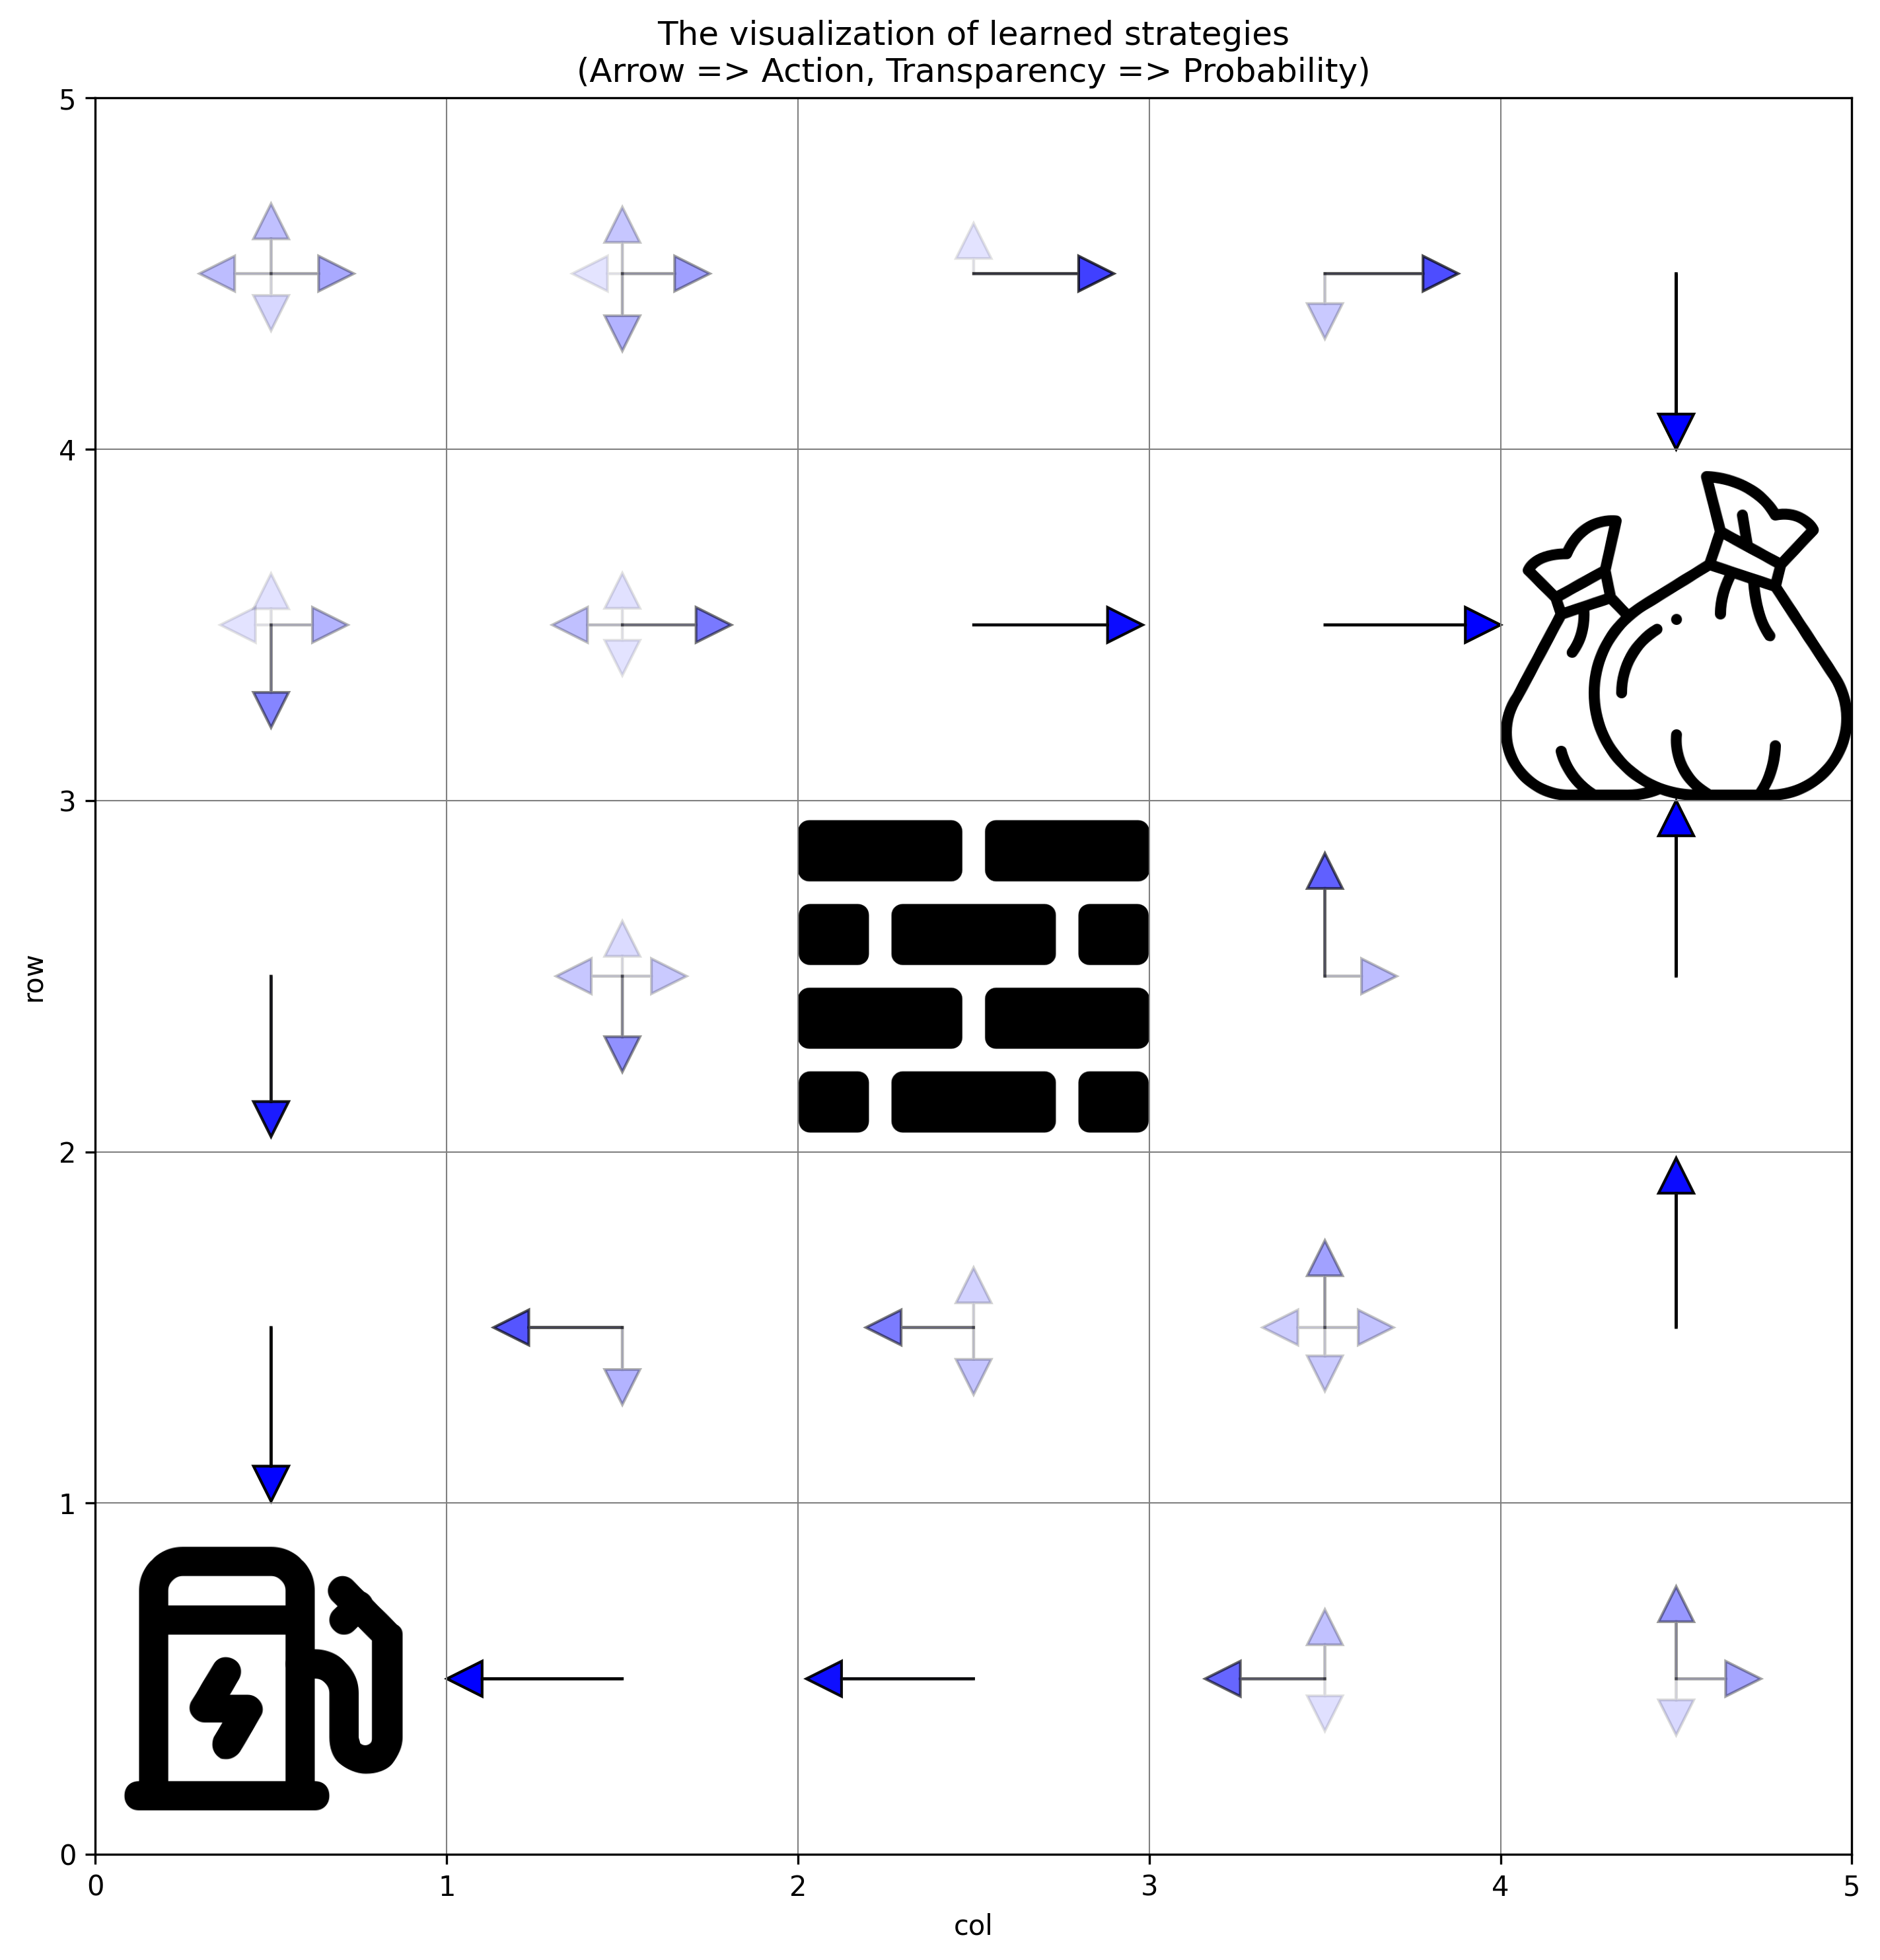
\includegraphics[width=0.5\textwidth]{figure/sweep_robot/REINFORCE/policy_visualization.png} 
    \caption{REINFORCE 策略梯度算法的策略可视化图}\label{fig:REINFORCE_policy} 
\end{figure}

\subsubsection{学习曲线}

本实验的学习曲线如图~\ref{fig:REINFORCE_training} 所示。我们展示了收益、步数和成功率的变化趋势。

\begin{figure}[htbp] 
    \centering 
    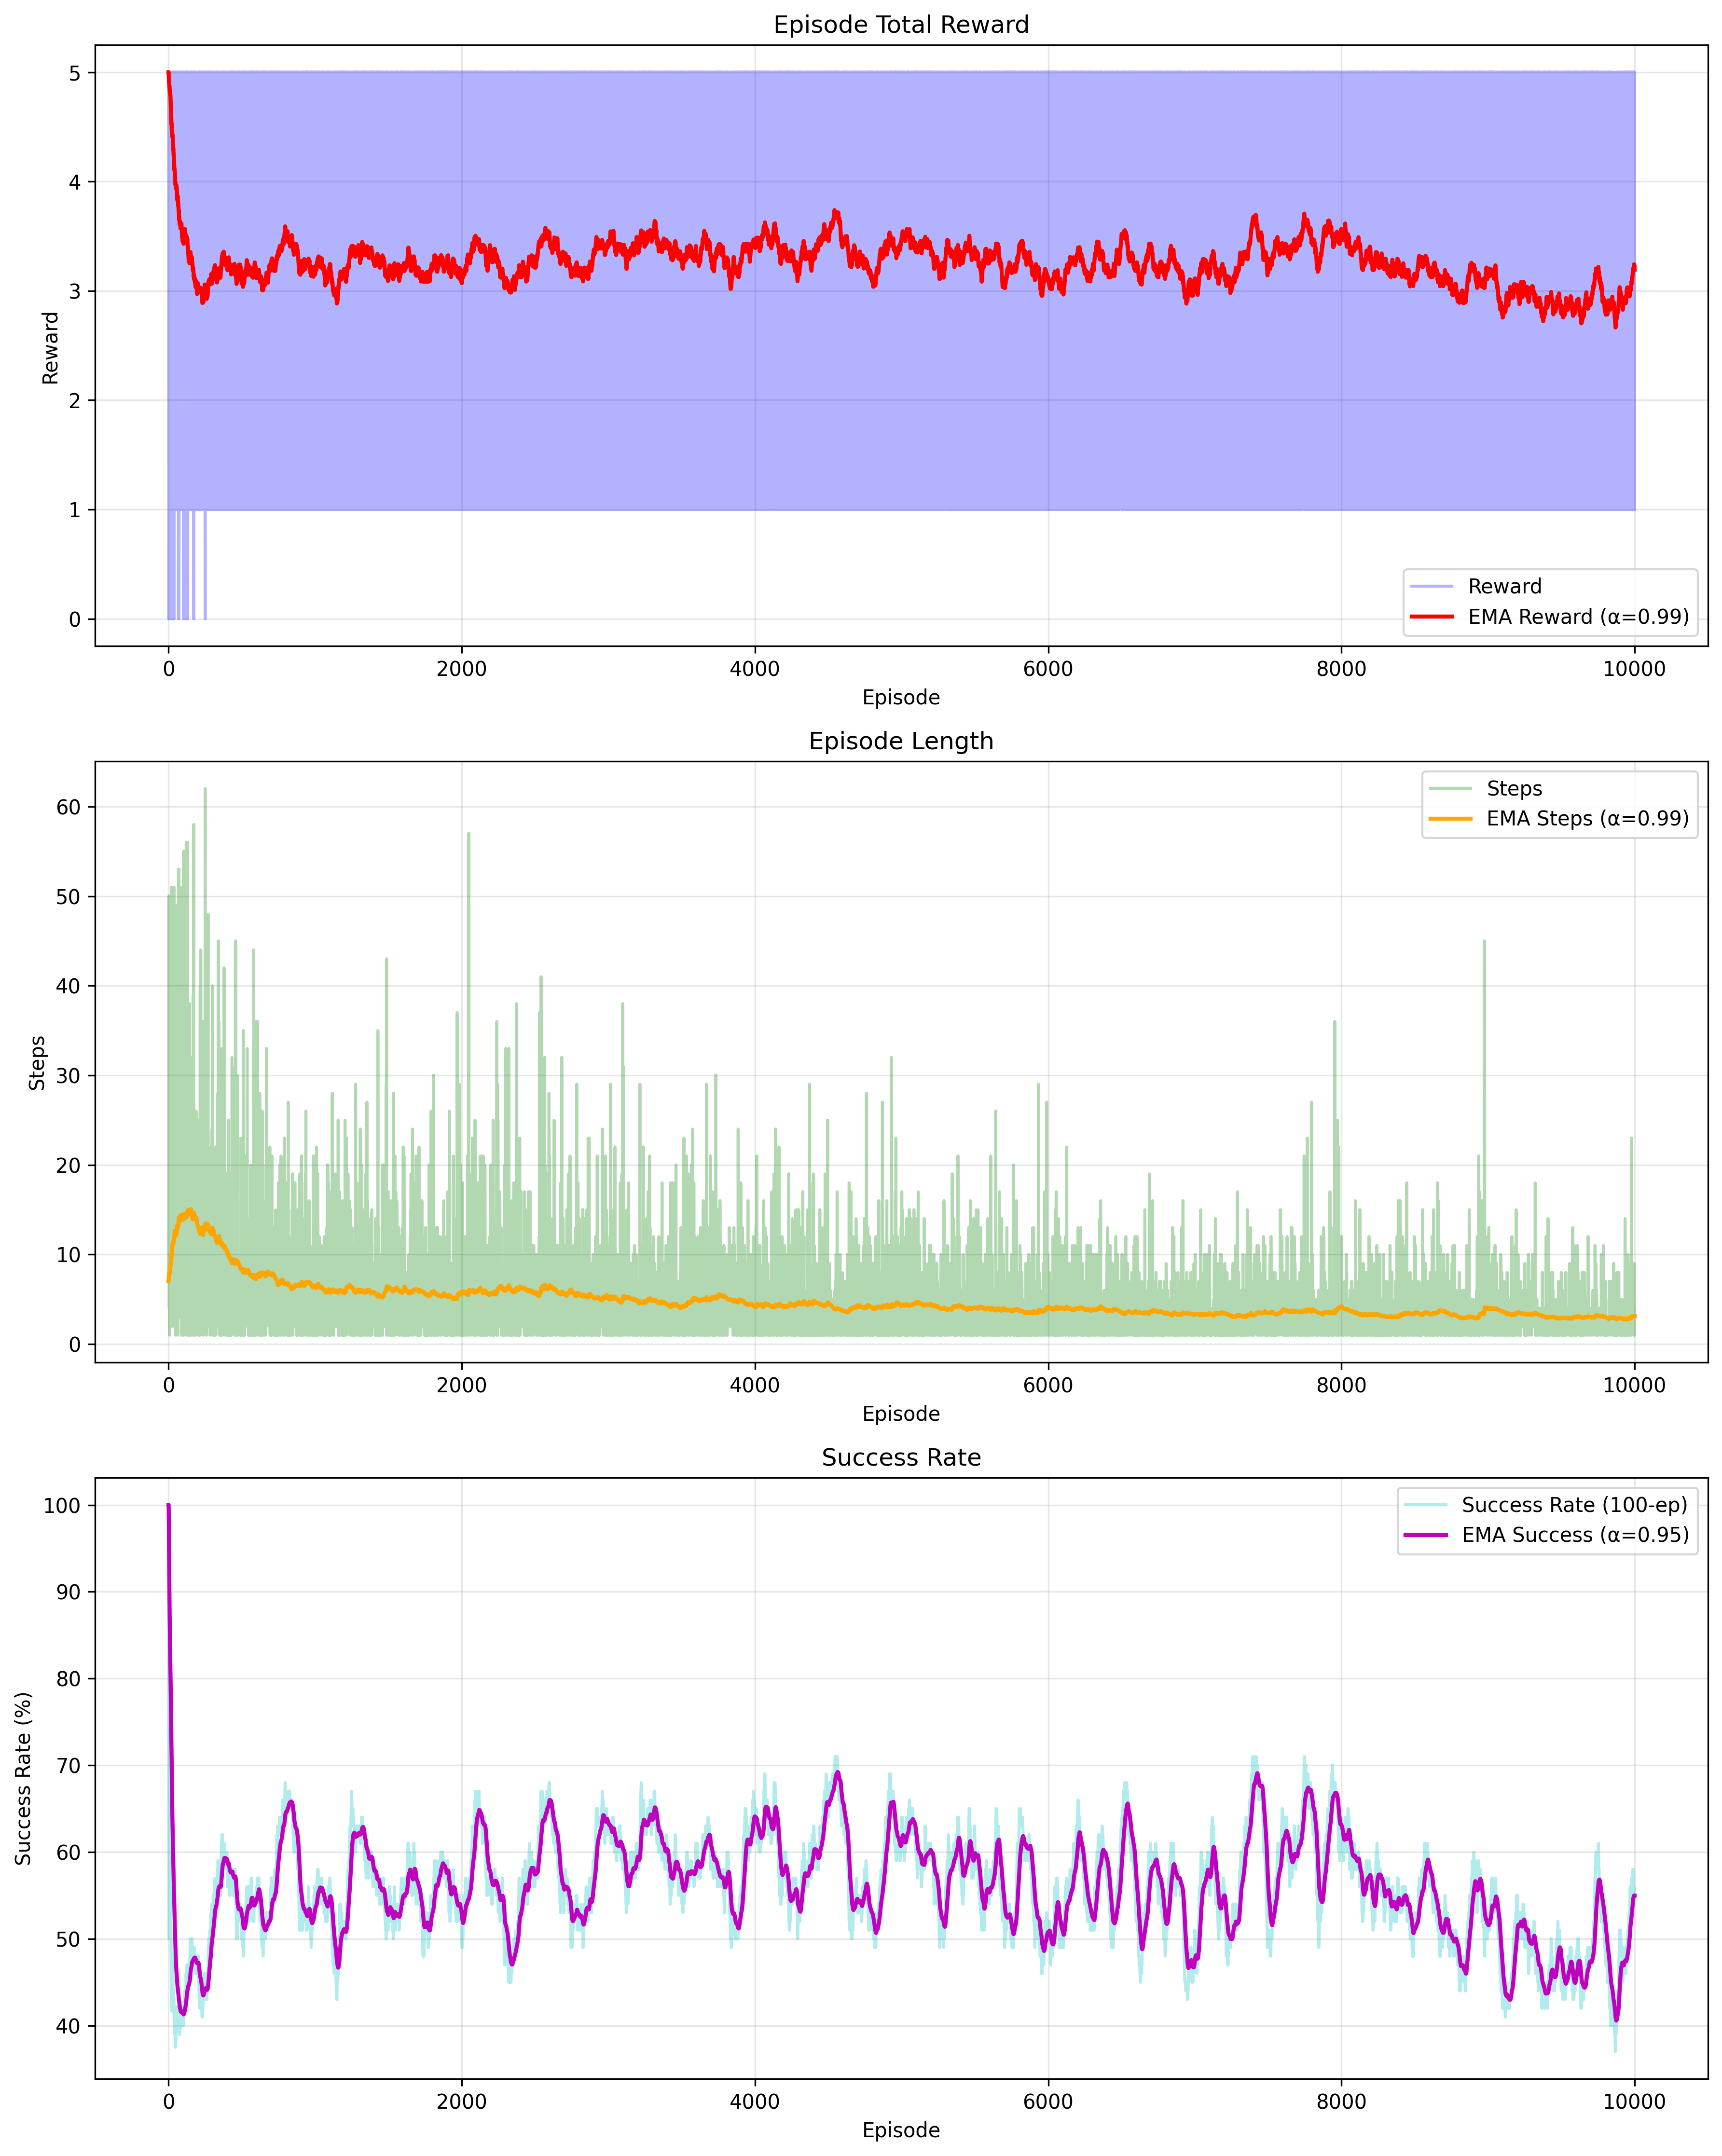
\includegraphics[width=0.8\textwidth]{figure/sweep_robot/REINFORCE/training_results.png} 
    \caption{REINFORCE 策略梯度算法的策略可视化图}\label{fig:REINFORCE_training} 
\end{figure}

可以发现,REINFORCE 算法在训练过程中,平均奖励水平较低,且波动较大。智能体在充电站附近停留时间过长,导致平均奖励水平未能有效提升,对于 SARAS 算法的表现较差。

\subsubsection{总结}

分析表明,REINFORCE 策略梯度算法在当前环境下未能习得有效的策略。
尽管智能体在训练过程中能够逐步收集垃圾,但其在充电站停留时间过长,导致平均奖励水平较低。
如图~\ref{fig:REINFORCE_policy} 所示,机器人越接近充电站,其选择充电而非收集垃圾的倾向越明显,这表明智能体可能在学习过程中陷入了局部最优解。

究其原因,核心问题在于环境奖励的稀疏性:仅在充电桩和垃圾位置提供奖励,使得智能体难以学习最优策略。其决策严重依赖轨迹末端状态,一旦习得“快速终止回合”的行为模式,便容易形成次优策略。

此外,REINFORCE 算法固有的特性也加剧了这一问题:
\begin{itemize}
    \item  \textbf{反馈延迟}:算法需等待整个回合结束后才能获得总回报。中间决策的优劣无法即时反馈给智能体。智能体需待回合结束方能评估决策正确性,这导致了难以识别关键决策。在奖励稀疏或环境复杂的情况下,这显著增加了陷入次优策略的风险。
    \item \textbf{稀疏奖励}:在仅终点(垃圾/充电桩)提供奖励的稀疏环境下,智能体需经历较长路径才能获得有效信息,极易因探索不足而固守次优策略。
    \item \textbf{更新噪声与不稳定性}:依赖整条轨迹回报进行全局更新,使得梯度易受随机噪声干扰,导致训练过程波动较大,难以收敛至全局最优策略。
\end{itemize}

REINFORCE 算法在这种环境下的收敛速度较慢,且容易受到高方差的影响,导致学习不稳定。